\setcounter{section}{9}
\section{Lineare Differentialgleichungssysteme}

\subsection{Homogene lineare Differentialgleichungen 1.\ Ordnung mit konstanten Koeffizienten}

Solche Gleichungen sind bereits aus der Analysis bekannt. Allgemein ist eine solche Differentialgleichung gegeben durch

\begin{equation*}
    y'(t)=ay(t), \quad a \in \mathbb{R}.
\end{equation*}

Mit der Lösung

\begin{equation*}
    y(t)= y(0) \ e^{at}.
\end{equation*}

Wobei \( y(0) \) die Anfangsbedingung ist. Ein konkretes Beispiel hierfür ist die Differentialgleichung

\begin{equation*}
    y'(t)=-2y(t),\  y(0) = 3.
\end{equation*}

Die Lösung ist dann gegeben durch 

\begin{figure*}[h]
    \centering
    \begin{minipage}
        {0.5\textwidth}
        \begin{equation*}
            y(t) = y(0) e^{-2t} = 3 e^{-2t}.
        \end{equation*}        
    \end{minipage}
    \hfill
    \begin{minipage}
        {0.45\textwidth}
        \centering
        \tikzsetnextfilename{lin_diff_01}
        \begin{tikzpicture}
            \begin{axis}[
                width = 5cm,
                axis lines = middle,
                xlabel = {t},
                ylabel = {y},
                xlabel style={below right},
                ylabel style={above}, 
                xmin=-0.5, xmax=4.5,
                % ymin=0, ymax=3.5,
                axis equal,
                xtick=\empty,
                ytick=\empty,
            ]
            \addplot [
                domain=-0.25:4, 
                samples=40, 
                color=red,
                thick, 
            ]
            { 3 *exp(-2*x) };
            % \node[pin={[pin edge={<-, thick, black}]right:{\( b \)}}] at (axis cs:0,1,0) {};
            \end{axis}
        \end{tikzpicture}
    \end{minipage}
\end{figure*}

Die Lösungsmenge dieser Differentialgleichung \( \left\{ y \in C^1(\mathbb{R}): y' = ay \right\} \) ist ein 1-D Unterraum von den 1-mal stetig differenzierbaren Funktionen \( C^1(\mathbb{R}) \).

\subsection{Systeme homogener linearer Differentialgleichungen 1.\ Ordnung mit konstanten Koeffizienten}

In der linearen Algebra I haben wir bereits gesehen wie wir Systeme von Gleichungen lösen und manipulieren können. Das geht auch mit Differentialgleichungen. Ein Beispiel dafür wäre zum Beispiel das Gleichungssystem gegeben durch

\vspace{1\baselineskip}

\begin{equation*}
    \left\{ 
        \begin{aligned}
            y_1'(t) &= -2 y_1(t), \quad y_1(0) = 1 \\
            y_2'(t) &= -4 y_2(t), \quad y_2(0) = 3. \\
        \end{aligned}
    \right.
\end{equation*}

\vspace{0.5\baselineskip}

Da beide Gleichungen von unterschiedlichen Variablen abhängen und dadurch unabhängig voneinander sind, nennen wir ein solches System entkoppelt. In einem solchen entkoppelten System können wir die Differentialgleichungen separat voneinander lösen. 

\newpage

\begin{figure*}[h]
    \centering
    \begin{minipage}
        {0.5\textwidth}
        \begin{equation*}
            \textcolor{customblue}{y_1(t)} = y_1(0) e^{-2t} = e^{-2t}
        \end{equation*}        
    \end{minipage}
    \hfill
    \begin{minipage}
        {0.45\textwidth}
        \centering
        \tikzsetnextfilename{lin_diff_02}
        \begin{tikzpicture}
            \begin{axis}[
                width = 5cm,
                axis lines = middle,
                xlabel = {t},
                ylabel = {\( y_1 \)},
                xlabel style={below right},
                ylabel style={above}, 
                xmin=-0.5, xmax=2.5,
                ymin=-0.5, ymax=3.5,
                % axis equal,
                xtick=\empty,
                ytick=\empty,
            ]
            \addplot [
                domain=0:2.25, 
                samples=40, 
                color=blue,
                thick, 
            ]
            { exp(-2*x) };
            % \node[pin={[pin edge={<-, thick, black}]right:{\( b \)}}] at (axis cs:0,1,0) {};
            \end{axis}
        \end{tikzpicture}
    \end{minipage}
\end{figure*}

\begin{figure*}[h]
    \centering
    \begin{minipage}
        {0.5\textwidth}
        \begin{equation*}
            \textcolor{customred}{y_2(t)} = y_2(0) e^{-4t} = 3 e^{-4t}
        \end{equation*}        
    \end{minipage}
    \hfill
    \begin{minipage}
        {0.45\textwidth}
        \centering
        \tikzsetnextfilename{lin_diff_03}
        \begin{tikzpicture}
            \begin{axis}[
                width = 5cm,
                axis lines = middle,
                xlabel = {t},
                ylabel = {\( y_2 \)},
                xlabel style={below right},
                ylabel style={above}, 
                xmin=-0.5, xmax=2.5,
                ymin=-0.5, ymax=3.5,
                % axis equal,
                xtick=\empty,
                ytick=\empty,
            ]
            \addplot [
                domain=0:2.25, 
                samples=40, 
                color=red,
                thick, 
            ]
            { 3 * exp(-4*x) };
            % \node[pin={[pin edge={<-, thick, black}]right:{\( b \)}}] at (axis cs:0,1,0) {};
            \end{axis}
        \end{tikzpicture}
    \end{minipage}
\end{figure*}

Wie bei den herkömmlichen LGS der Form \( Ax = b \), können wir auch dieses System von linearen Differentialgleichungen in Matrixform schreiben bloss, dass die allgemeine Form nun \( y' = Ay \) ist. In unserem Fall ergibt sich

\begin{equation*}
    \begin{pmatrix}
        y_1'(t) \\
        y_2'(t)
    \end{pmatrix} = 
    \begin{pmatrix}
        -2 & 0 \\
        0 & -4
    \end{pmatrix}
    \begin{pmatrix}
        y_1(t) \\
        y_2(t)
    \end{pmatrix},
    \quad \begin{pmatrix}
        y_1(0) \\
        y_2(0)
    \end{pmatrix} = y(0) =
    \begin{pmatrix}
        1 \\
        3
    \end{pmatrix}.
\end{equation*}

\vspace{0.25\baselineskip}

Die Lösung dieses Systems lässt sich dann als Vektor schreiben:

\begin{equation*}
    y(t) = 
    e^{-2t}
    \begin{pmatrix}
        1 \\
        0
    \end{pmatrix} +
    e^{-4t}
    \begin{pmatrix}
        0 \\
        3
    \end{pmatrix}.
\end{equation*}

\vspace{0.25\baselineskip}

Grafisch können wir uns die zusammengesetzte Lösung von \( y_1 \) und \( y_2 \) wie eine Linearkombination vorstellen, bloss das jetzt alles noch von \( t \) abhängt. 

\begin{figure}[h]
    \centering
    \tikzsetnextfilename{lin_diff_04}
    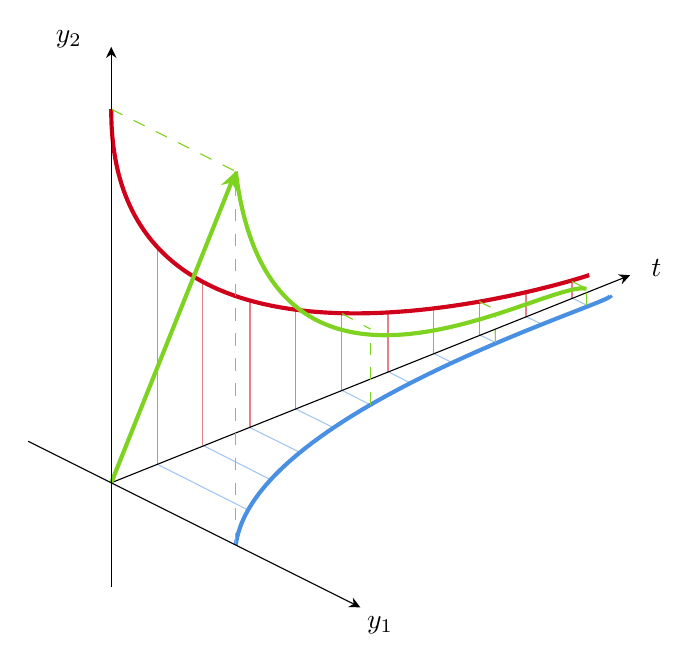
\begin{tikzpicture}[x=0.75pt,y=0.75pt,yscale=-1,xscale=1]
        %Straight Lines [id:da6266944733728231] 
        \draw [color={rgb, 255:red, 208; green, 2; blue, 27 }  ,draw opacity=0.5 ]   (242.33,147.17) -- (242.33,251.17) ;
        %Straight Lines [id:da9473718551797458] 
        \draw [color={rgb, 255:red, 208; green, 2; blue, 27 }  ,draw opacity=0.5 ]   (264.08,162.92) -- (264.08,241.92) ;
        %Straight Lines [id:da3375189209092121] 
        \draw [color={rgb, 255:red, 208; green, 2; blue, 27 }  ,draw opacity=0.5 ]   (286.83,172.42) -- (286.83,233.42) ;
        %Straight Lines [id:da585381201015521] 
        \draw [color={rgb, 255:red, 208; green, 2; blue, 27 }  ,draw opacity=0.5 ]   (308.83,176.42) -- (308.83,224.42) ;
        %Straight Lines [id:da989334182528751] 
        \draw [color={rgb, 255:red, 208; green, 2; blue, 27 }  ,draw opacity=0.5 ]   (331.08,178.42) -- (331.08,215.42) ;
        %Straight Lines [id:da21157481547876977] 
        \draw [color={rgb, 255:red, 208; green, 2; blue, 27 }  ,draw opacity=0.5 ]   (353.33,178.42) -- (353.33,206.42) ;
        %Straight Lines [id:da6750318344383669] 
        \draw [color={rgb, 255:red, 208; green, 2; blue, 27 }  ,draw opacity=0.5 ]   (375.33,175.67) -- (375.33,197.67) ;
        %Straight Lines [id:da07171771142136829] 
        \draw [color={rgb, 255:red, 208; green, 2; blue, 27 }  ,draw opacity=0.5 ]   (397.33,172.67) -- (397.33,188.67) ;
        %Straight Lines [id:da4075047389571379] 
        \draw [color={rgb, 255:red, 208; green, 2; blue, 27 }  ,draw opacity=0.5 ]   (419.83,167.92) -- (419.83,179.92) ;
        %Straight Lines [id:da6591683928404128] 
        \draw [color={rgb, 255:red, 208; green, 2; blue, 27 }  ,draw opacity=0.5 ]   (442,163) -- (442,171) ;
        %Straight Lines [id:da9909465982671221] 
        \draw [color={rgb, 255:red, 74; green, 144; blue, 226 }  ,draw opacity=0.5 ]   (242.33,251.17) -- (286.25,273.25) ;
        %Straight Lines [id:da3756346843414533] 
        \draw [color={rgb, 255:red, 74; green, 144; blue, 226 }  ,draw opacity=0.5 ]   (264.08,241.92) -- (297.08,258.67) ;
        %Straight Lines [id:da9777741491261767] 
        \draw [color={rgb, 255:red, 74; green, 144; blue, 226 }  ,draw opacity=0.5 ]   (286.83,233.42) -- (311.08,245.42) ;
        %Straight Lines [id:da21510571632197606] 
        \draw [color={rgb, 255:red, 74; green, 144; blue, 226 }  ,draw opacity=0.5 ]   (308.83,224.42) -- (327.58,233.67) ;
        %Straight Lines [id:da5494003280478376] 
        \draw [color={rgb, 255:red, 74; green, 144; blue, 226 }  ,draw opacity=0.5 ]   (331.08,215.42) -- (344.83,222.42) ;
        %Straight Lines [id:da8304348712132449] 
        \draw [color={rgb, 255:red, 74; green, 144; blue, 226 }  ,draw opacity=0.5 ]   (353.33,206.42) -- (364.58,212.17) ;
        %Straight Lines [id:da10249677615168695] 
        \draw [color={rgb, 255:red, 74; green, 144; blue, 226 }  ,draw opacity=0.5 ]   (375.33,197.67) -- (384.33,202.17) ;
        %Straight Lines [id:da33625113634117754] 
        \draw [color={rgb, 255:red, 74; green, 144; blue, 226 }  ,draw opacity=0.5 ]   (397.33,188.67) -- (405.08,192.42) ;
        %Straight Lines [id:da4720358563705469] 
        \draw [color={rgb, 255:red, 74; green, 144; blue, 226 }  ,draw opacity=0.5 ]   (419.83,179.92) -- (427.08,183.42) ;
        %Straight Lines [id:da3548721469063173] 
        \draw [color={rgb, 255:red, 74; green, 144; blue, 226 }  ,draw opacity=0.5 ]   (441.83,170.92) -- (449.08,174.42) ;
        %Straight Lines [id:da17981019374494978] 
        \draw    (220,260) -- (467.21,161.11) ;
        \draw [shift={(470,160)}, rotate = 158.2] [fill={rgb, 255:red, 0; green, 0; blue, 0 }  ][line width=0.08]  [draw opacity=0] (5.36,-2.57) -- (0,0) -- (5.36,2.57) -- (3.56,0) -- cycle    ;
        %Curve Lines [id:da2959295993490375] 
        \draw [color={rgb, 255:red, 74; green, 144; blue, 226 }  ,draw opacity=1 ][line width=1.5]    (460,170) .. controls (468.42,171.25) and (288.5,224.5) .. (280,290) ;
        %Curve Lines [id:da9691686052962586] 
        \draw [color={rgb, 255:red, 208; green, 2; blue, 27 }  ,draw opacity=1 ][line width=1.5]    (450,160) .. controls (460,157) and (219.33,238.67) .. (220,80) ;
        %Straight Lines [id:da21487560786590698] 
        \draw [color={rgb, 255:red, 126; green, 211; blue, 33 }  ,draw opacity=1 ] [dash pattern={on 4.5pt off 4.5pt}]  (220,80) -- (280,110) ;
        %Straight Lines [id:da7887659673436868] 
        \draw [color={rgb, 255:red, 126; green, 211; blue, 33 }  ,draw opacity=1 ] [dash pattern={on 4.5pt off 4.5pt}]  (280,290) -- (280,110) ;
        %Straight Lines [id:da09158980326810207] 
        \draw [color={rgb, 255:red, 126; green, 211; blue, 33 }  ,draw opacity=1 ] [dash pattern={on 4.5pt off 4.5pt}]  (344.83,222.42) -- (344.83,188.67) ;
        %Straight Lines [id:da5344220902516645] 
        \draw [color={rgb, 255:red, 126; green, 211; blue, 33 }  ,draw opacity=1 ] [dash pattern={on 4.5pt off 4.5pt}]  (331.08,178.42) -- (345,186) ;
        %Straight Lines [id:da7246234521000464] 
        \draw [color={rgb, 255:red, 126; green, 211; blue, 33 }  ,draw opacity=1 ] [dash pattern={on 4.5pt off 4.5pt}]  (405.08,192.42) -- (404.92,178.5) ;
        %Straight Lines [id:da30101186267489277] 
        \draw [color={rgb, 255:red, 126; green, 211; blue, 33 }  ,draw opacity=1 ] [dash pattern={on 4.5pt off 4.5pt}]  (397.33,172.67) -- (404.92,176.5) ;
        %Curve Lines [id:da25368345747771415] 
        \draw [color={rgb, 255:red, 126; green, 211; blue, 33 }  ,draw opacity=1 ][line width=1.5]    (280,110) .. controls (296.69,248.25) and (429.42,161.75) .. (449,166.5) ;
        %Straight Lines [id:da04224144437602262] 
        \draw [color={rgb, 255:red, 126; green, 211; blue, 33 }  ,draw opacity=1 ][line width=1.5]    (220,260) -- (278.51,113.71) ;
        \draw [shift={(280,110)}, rotate = 111.8] [fill={rgb, 255:red, 126; green, 211; blue, 33 }  ,fill opacity=1 ][line width=0.08]  [draw opacity=0] (8.75,-4.2) -- (0,0) -- (8.75,4.2) -- (5.81,0) -- cycle    ;
        %Straight Lines [id:da6973116866864064] 
        \draw    (220,310) -- (220,53) ;
        \draw [shift={(220,50)}, rotate = 90] [fill={rgb, 255:red, 0; green, 0; blue, 0 }  ][line width=0.08]  [draw opacity=0] (5.36,-2.57) -- (0,0) -- (5.36,2.57) -- (3.56,0) -- cycle    ;
        %Straight Lines [id:da19482417766302107] 
        \draw    (180,240) -- (337.32,318.66) ;
        \draw [shift={(340,320)}, rotate = 206.57] [fill={rgb, 255:red, 0; green, 0; blue, 0 }  ][line width=0.08]  [draw opacity=0] (5.36,-2.57) -- (0,0) -- (5.36,2.57) -- (3.56,0) -- cycle    ;
        %Straight Lines [id:da5500107339514307] 
        \draw [color={rgb, 255:red, 126; green, 211; blue, 33 }  ,draw opacity=1 ] [dash pattern={on 4.5pt off 4.5pt}]  (449.08,174.42) -- (448.92,166.5) ;
        %Straight Lines [id:da1413956810230076] 
        \draw [color={rgb, 255:red, 126; green, 211; blue, 33 }  ,draw opacity=1 ] [dash pattern={on 4.5pt off 4.5pt}]  (442,163) -- (449.58,166.83) ;

        % Text Node
        \draw (342,323) node [anchor=north west][inner sep=0.75pt]   [align=left] {$\displaystyle y_{1}$};
        % Text Node
        \draw (192,41) node [anchor=north west][inner sep=0.75pt]   [align=left] {$\displaystyle y_{2}$};
        % Text Node
        \draw (479,151) node [anchor=north west][inner sep=0.75pt]   [align=left] {$\displaystyle t$};

    \end{tikzpicture}
\end{figure}

Es kann aber auch sein, dass die Differentialgleichungen nicht entkoppelt sind. In dem Fall sind die Gleichungen voneinander abhängig und wir können sie nicht mehr separat lösen. Ein Beispiel dafür wäre das Gleichungssystem

\begin{equation*}
    \left\{ 
        \begin{aligned}
            y_1'(t) &= -4 y_1(t) - y_2(t) \\
            y_2'(t) &= -2 y_1(t) - 3 y_2(t)
        \end{aligned}
    \right. \quad \longrightarrow \quad
    \underbrace{\begin{pmatrix}
        y_1'(t) \\
        y_2'(t)
    \end{pmatrix} =
    \begin{pmatrix}
        -4 & -1 \\
        -2 & -3
    \end{pmatrix}
    \begin{pmatrix}
        y_1(t) \\
        y_2(t)
    \end{pmatrix}}_{\text{nicht direkt lösbar}}, \quad y(0)=
    \begin{pmatrix}
        1 \\
        3
    \end{pmatrix}.
\end{equation*}

Es stellt sich nun die Frage wie wir ein solches System dennoch lösen können. Betrachten wir dafür nochmals genauer die Matrizen \( A_1\) und \( A_2 \) der beiden Systeme.

\begin{equation*}
    A_1 = \begin{pmatrix}
        -2 & 0 \\
        0 & -4
    \end{pmatrix}, \quad
    A_2 = \begin{pmatrix}
        -4 & -1 \\
        -2 & -3
    \end{pmatrix}.
\end{equation*}

Wir erkennen, dass die Matrix \( A_1 \) des entkoppelten Systems diagonal ist. Im Rückschluss können wir also für das zweite System eine Lösung finden, indem wir einen Basiswechsel \( y = Tz \) durchführen und dadurch die Matrix \( A_2 \) diagonalisieren. Wir transformieren also das gesamte Gleichungssystem in die Eigenbasis von \( A_2 \). Dafür benötigen wir die Eigenwerte und Eigenvektoren, welche die Spalten unserer Transformationsmatrix \( T \) bilden.   

\begin{equation*}
    \lambda_1 = -2, \quad \lambda_2 = -5, \quad T = \begin{pmatrix}
        -\frac{1}{2} & 1 \\
        1 & 1
    \end{pmatrix}, \quad T^{-1} = \frac{1}{3} \begin{pmatrix}
        -2 & 2 \\
        2 & 1
    \end{pmatrix}.
\end{equation*}

Nun können wir die Transformation durchführen. 

\begin{equation*}
        \begin{aligned}
            \begin{pmatrix}
                y_1'(t) \\
                y_2'(t)
            \end{pmatrix} &=
            \begin{pmatrix}
                -4 & -1 \\
                -2 & -3
            \end{pmatrix}
            \begin{pmatrix}
                y_1(t) \\
                y_2(t)
            \end{pmatrix} \\[0.5em]
            y(0)&= \begin{pmatrix}
                y_1(0) \\
                y_2(0)
            \end{pmatrix}
            \begin{pmatrix}
                1 \\
                3
            \end{pmatrix} 
        \end{aligned} \quad \xRightarrow{y = Tz} \quad
        \begin{aligned}
            \begin{pmatrix}
                z_1'(t) \\
                z_2'(t)
            \end{pmatrix} &=
            \underbrace{\begin{pmatrix}
                -2 & 0 \\
                0 & -5
            \end{pmatrix}}_{T^{-1} A T}
            \begin{pmatrix}
                z_1(t) \\
                z_2(t)
            \end{pmatrix} \\[0.5em]
            z(0)&= \begin{pmatrix}
                z_1(0) \\
                z_2(0)
            \end{pmatrix} =
            \underbrace{\begin{pmatrix}
                \frac{4}{3} \\
                \frac{5}{3}
            \end{pmatrix}}_{T^{-1} y(0)}
        \end{aligned}
\end{equation*}

In der Basis \( z \) können wir das Problem nun wie oben entkoppelt lösen 

\begin{equation*}
    z(t) = 
    \begin{pmatrix}
        \frac{4}{3} \\
        0
    \end{pmatrix} e^{-2t} +
    \begin{pmatrix}
        0 \\
        \frac{5}{3}
    \end{pmatrix} e^{-5t} ,
\end{equation*}

und danach wieder mit \( y = Tz \) zurücktransformieren.

\begin{equation*}
    \begin{aligned}
        y(t) &= 
        \underbrace{\begin{pmatrix}
            -\frac{1}{2} & 1 \\
            1 & 1
        \end{pmatrix}
        \begin{pmatrix}
            \frac{4}{3} \\
            0
        \end{pmatrix}}_{z_1(0) t^{(1)}} e^{-2t} + 
        \underbrace{\begin{pmatrix}
            -\frac{1}{2} & 1 \\
            1 & 1
        \end{pmatrix}
        \begin{pmatrix}
            0 \\
            \frac{5}{3}
        \end{pmatrix}}_{z_2(0) t^{(2)}} e^{-5t} \\[0.5em]
        &= \frac{4}{3} \begin{pmatrix}
            -\frac{1}{2} \\ 1
        \end{pmatrix} e^{-2t} + \frac{5}{3} \begin{pmatrix}
            1 \\ 1
        \end{pmatrix} e^{-5t} \\[0.5em]
        &= \frac{1}{3} \begin{pmatrix}
            -2 e^{-2t} + 5 e^{-5t} \\
            4 e^{-2t} + 5 e^{-5t}
        \end{pmatrix} 
    \end{aligned}
\end{equation*}

\newpage

\begin{figure*}[h]
    \centering
    \tikzsetnextfilename{lin_diff_05}
    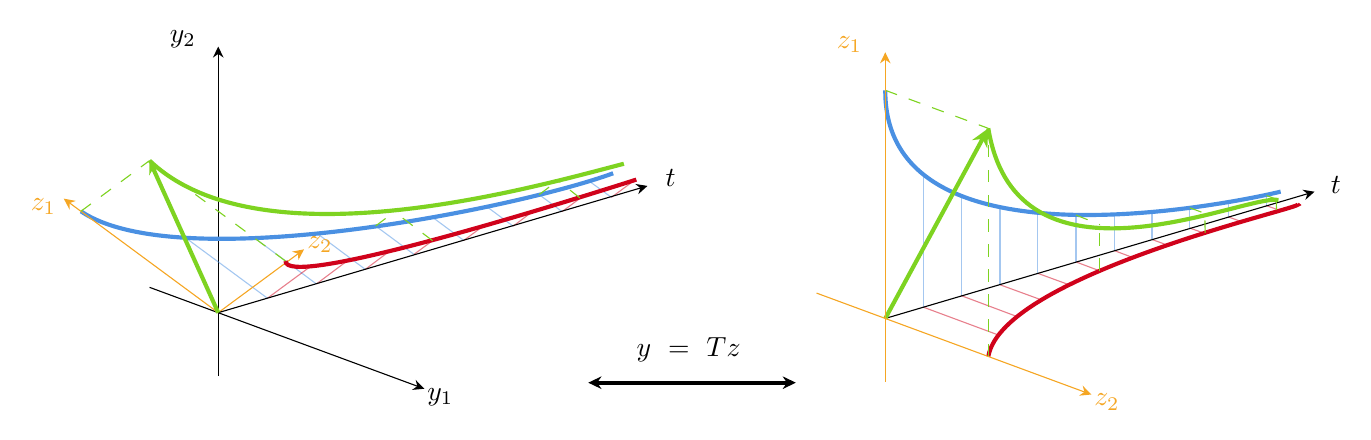
\begin{tikzpicture}[x=0.75pt,y=0.75pt,yscale=-1,xscale=1]
        %Straight Lines [id:da6973116866864064] 
        \draw    (101.71,176.81) -- (101.71,21.03) ;
        \draw [shift={(101.71,18.03)}, rotate = 90] [fill={rgb, 255:red, 0; green, 0; blue, 0 }  ][line width=0.08]  [draw opacity=0] (5.36,-2.57) -- (0,0) -- (5.36,2.57) -- (3.56,0) -- cycle    ;
        %Straight Lines [id:da19482417766302107] 
        \draw    (68.62,134.06) -- (198.16,181.88) ;
        \draw [shift={(200.97,182.92)}, rotate = 200.26] [fill={rgb, 255:red, 0; green, 0; blue, 0 }  ][line width=0.08]  [draw opacity=0] (5.36,-2.57) -- (0,0) -- (5.36,2.57) -- (3.56,0) -- cycle    ;
        %Curve Lines [id:da08513489705436428] 
        \draw [color={rgb, 255:red, 74; green, 144; blue, 226 }  ,draw opacity=1 ][line width=1.5]    (35.53,97.42) .. controls (83.1,129.48) and (247.78,95.38) .. (291.97,79.1) ;
        %Straight Lines [id:da480194643171141] 
        \draw [color={rgb, 255:red, 74; green, 144; blue, 226 }  ,draw opacity=0.5 ]   (85.72,109.99) -- (125.42,139.3) ;
        %Straight Lines [id:da8765916105340299] 
        \draw [color={rgb, 255:red, 74; green, 144; blue, 226 }  ,draw opacity=0.5 ]   (119.22,110.29) -- (149,132.43) ;
        %Straight Lines [id:da9016984831718732] 
        \draw [color={rgb, 255:red, 74; green, 144; blue, 226 }  ,draw opacity=0.5 ]   (149.2,108) -- (172.57,125.41) ;
        %Straight Lines [id:da06527674628340907] 
        \draw [color={rgb, 255:red, 74; green, 144; blue, 226 }  ,draw opacity=0.5 ]   (177.54,104.49) -- (196.01,118.18) ;
        %Straight Lines [id:da15053306290824608] 
        \draw [color={rgb, 255:red, 74; green, 144; blue, 226 }  ,draw opacity=0.5 ]   (204.83,100.22) -- (220,111.46) ;
        %Straight Lines [id:da6444258607159444] 
        \draw [color={rgb, 255:red, 74; green, 144; blue, 226 }  ,draw opacity=0.5 ]   (230.89,95.03) -- (243.78,104.59) ;
        %Straight Lines [id:da21726565860540858] 
        \draw [color={rgb, 255:red, 74; green, 144; blue, 226 }  ,draw opacity=0.5 ]   (256.33,89.38) -- (267.36,97.57) ;
        %Straight Lines [id:da04470688703996384] 
        \draw [color={rgb, 255:red, 74; green, 144; blue, 226 }  ,draw opacity=0.5 ]   (280.32,82.81) -- (291.14,90.7) ;
        %Straight Lines [id:da7191672671487107] 
        \draw [color={rgb, 255:red, 245; green, 166; blue, 35 }  ,draw opacity=1 ]   (101.71,146.27) -- (140.66,117.52) ;
        \draw [shift={(143.07,115.74)}, rotate = 143.56] [fill={rgb, 255:red, 245; green, 166; blue, 35 }  ,fill opacity=1 ][line width=0.08]  [draw opacity=0] (5.36,-2.57) -- (0,0) -- (5.36,2.57) -- (3.56,0) -- cycle    ;
        %Straight Lines [id:da4185604234445439] 
        \draw [color={rgb, 255:red, 245; green, 166; blue, 35 }  ,draw opacity=1 ]   (101.71,146.27) -- (29.67,93.09) ;
        \draw [shift={(27.26,91.31)}, rotate = 36.44] [fill={rgb, 255:red, 245; green, 166; blue, 35 }  ,fill opacity=1 ][line width=0.08]  [draw opacity=0] (5.36,-2.57) -- (0,0) -- (5.36,2.57) -- (3.56,0) -- cycle    ;
        %Straight Lines [id:da2110224209161562] 
        \draw [color={rgb, 255:red, 208; green, 2; blue, 27 }  ,draw opacity=0.5 ]   (145.21,124.7) -- (125.42,139.3) ;
        %Straight Lines [id:da5401560194775785] 
        \draw [color={rgb, 255:red, 208; green, 2; blue, 27 }  ,draw opacity=0.5 ]   (162.99,121.95) -- (149,132.43) ;
        %Straight Lines [id:da8222227187807968] 
        \draw [color={rgb, 255:red, 208; green, 2; blue, 27 }  ,draw opacity=0.5 ]   (183.05,117.52) -- (172.57,125.41) ;
        %Straight Lines [id:da3066984749171462] 
        \draw [color={rgb, 255:red, 208; green, 2; blue, 27 }  ,draw opacity=0.5 ]   (204.97,111.57) -- (196.01,118.18) ;
        %Straight Lines [id:da5247959408524067] 
        \draw [color={rgb, 255:red, 208; green, 2; blue, 27 }  ,draw opacity=0.5 ]   (228.96,104.85) -- (220,111.46) ;
        %Straight Lines [id:da33804442139226776] 
        \draw [color={rgb, 255:red, 208; green, 2; blue, 27 }  ,draw opacity=0.5 ]   (253.36,97.37) -- (243.78,104.59) ;
        %Straight Lines [id:da6967033383862246] 
        \draw [color={rgb, 255:red, 208; green, 2; blue, 27 }  ,draw opacity=0.5 ]   (277.56,90.04) -- (267.36,97.57) ;
        %Curve Lines [id:da47234430544916095] 
        \draw [color={rgb, 255:red, 208; green, 2; blue, 27 }  ,draw opacity=1 ][line width=1.5]    (134.11,121.36) .. controls (133.69,134.8) and (257.22,96.81) .. (303.14,82.15) ;
        %Straight Lines [id:da569875452358045] 
        \draw [color={rgb, 255:red, 208; green, 2; blue, 27 }  ,draw opacity=0.5 ]   (301.34,83.17) -- (291.14,90.7) ;
        %Straight Lines [id:da17981019374494978] 
        \draw    (101.71,146.27) -- (305.63,86.05) ;
        \draw [shift={(308.51,85.2)}, rotate = 163.55] [fill={rgb, 255:red, 0; green, 0; blue, 0 }  ][line width=0.08]  [draw opacity=0] (5.36,-2.57) -- (0,0) -- (5.36,2.57) -- (3.56,0) -- cycle    ;
        %Straight Lines [id:da9415269093479173] 
        \draw [color={rgb, 255:red, 126; green, 211; blue, 33 }  ,draw opacity=1 ] [dash pattern={on 4.5pt off 4.5pt}]  (134.11,121.36) -- (68.62,72.99) ;
        %Straight Lines [id:da15516610453542312] 
        \draw [color={rgb, 255:red, 126; green, 211; blue, 33 }  ,draw opacity=1 ] [dash pattern={on 4.5pt off 4.5pt}]  (35.53,97.42) -- (68.62,72.99) ;
        %Straight Lines [id:da4776364310806127] 
        \draw [color={rgb, 255:red, 126; green, 211; blue, 33 }  ,draw opacity=1 ][line width=1.5]    (101.71,146.27) -- (70.27,76.64) ;
        \draw [shift={(68.62,72.99)}, rotate = 65.7] [fill={rgb, 255:red, 126; green, 211; blue, 33 }  ,fill opacity=1 ][line width=0.08]  [draw opacity=0] (6.43,-3.09) -- (0,0) -- (6.43,3.09) -- (4.27,0) -- cycle    ;
        %Straight Lines [id:da653342410886829] 
        \draw [color={rgb, 255:red, 126; green, 211; blue, 33 }  ,draw opacity=1 ] [dash pattern={on 4.5pt off 4.5pt}]  (204.97,111.57) -- (186.57,97.67) ;
        %Straight Lines [id:da7466676557543097] 
        \draw [color={rgb, 255:red, 126; green, 211; blue, 33 }  ,draw opacity=1 ] [dash pattern={on 4.5pt off 4.5pt}]  (177.54,104.49) -- (186.57,97.67) ;
        %Straight Lines [id:da696671503270543] 
        \draw [color={rgb, 255:red, 126; green, 211; blue, 33 }  ,draw opacity=1 ] [dash pattern={on 4.5pt off 4.5pt}]  (256.33,89.38) -- (265.36,82.56) ;
        %Straight Lines [id:da20878230287791089] 
        \draw [color={rgb, 255:red, 126; green, 211; blue, 33 }  ,draw opacity=1 ] [dash pattern={on 4.5pt off 4.5pt}]  (275.91,90.96) -- (265.36,82.56) ;
        %Curve Lines [id:da0965297607342761] 
        \draw [color={rgb, 255:red, 126; green, 211; blue, 33 }  ,draw opacity=1 ][line width=1.5]    (68.62,72.99) .. controls (121.77,123.83) and (254.74,85.51) .. (297.14,74.52) ;
        %Straight Lines [id:da732954561581312] 
        \draw [color={rgb, 255:red, 74; green, 144; blue, 226 }  ,draw opacity=0.5 ]   (441.56,80.15) -- (441.56,143.66) ;
        %Straight Lines [id:da461504352207845] 
        \draw [color={rgb, 255:red, 74; green, 144; blue, 226 }  ,draw opacity=0.5 ]   (460,90) -- (460,138.25) ;
        %Straight Lines [id:da5183412242892095] 
        \draw [color={rgb, 255:red, 74; green, 144; blue, 226 }  ,draw opacity=0.5 ]   (478.37,95.57) -- (478.37,132.82) ;
        %Straight Lines [id:da694355332751654] 
        \draw [color={rgb, 255:red, 74; green, 144; blue, 226 }  ,draw opacity=0.5 ]   (496.57,98.01) -- (496.57,127.32) ;
        %Straight Lines [id:da7036925222416096] 
        \draw [color={rgb, 255:red, 74; green, 144; blue, 226 }  ,draw opacity=0.5 ]   (514.98,99.23) -- (514.98,121.83) ;
        %Straight Lines [id:da7106406909226872] 
        \draw [color={rgb, 255:red, 74; green, 144; blue, 226 }  ,draw opacity=0.5 ]   (533.38,99.23) -- (533.38,116.33) ;
        %Straight Lines [id:da7982276024443253] 
        \draw [color={rgb, 255:red, 74; green, 144; blue, 226 }  ,draw opacity=0.5 ]   (551.58,97.55) -- (551.58,110.99) ;
        %Straight Lines [id:da39772396010068467] 
        \draw [color={rgb, 255:red, 74; green, 144; blue, 226 }  ,draw opacity=0.5 ]   (569.78,95.72) -- (569.78,105.49) ;
        %Straight Lines [id:da9581463904164798] 
        \draw [color={rgb, 255:red, 74; green, 144; blue, 226 }  ,draw opacity=0.5 ]   (588.39,92.82) -- (588.39,100.15) ;
        %Straight Lines [id:da21230024411919568] 
        \draw [color={rgb, 255:red, 74; green, 144; blue, 226 }  ,draw opacity=0.5 ]   (606.73,89.81) -- (606.73,94.7) ;
        %Straight Lines [id:da12534114996282653] 
        \draw [color={rgb, 255:red, 208; green, 2; blue, 27 }  ,draw opacity=0.5 ]   (441.56,143.66) -- (477.89,157.14) ;
        %Straight Lines [id:da9852532904684287] 
        \draw [color={rgb, 255:red, 208; green, 2; blue, 27 }  ,draw opacity=0.5 ]   (459.55,138.01) -- (486.85,148.24) ;
        %Straight Lines [id:da13596538269564484] 
        \draw [color={rgb, 255:red, 208; green, 2; blue, 27 }  ,draw opacity=0.5 ]   (478.37,132.82) -- (498.43,140.15) ;
        %Straight Lines [id:da7957230622159118] 
        \draw [color={rgb, 255:red, 208; green, 2; blue, 27 }  ,draw opacity=0.5 ]   (496.57,127.32) -- (512.08,132.97) ;
        %Straight Lines [id:da036679710503269014] 
        \draw [color={rgb, 255:red, 208; green, 2; blue, 27 }  ,draw opacity=0.5 ]   (514.98,121.83) -- (526.35,126.1) ;
        %Straight Lines [id:da1434190340032383] 
        \draw [color={rgb, 255:red, 208; green, 2; blue, 27 }  ,draw opacity=0.5 ]   (533.38,116.33) -- (542.69,119.84) ;
        %Straight Lines [id:da3932956677007009] 
        \draw [color={rgb, 255:red, 208; green, 2; blue, 27 }  ,draw opacity=0.5 ]   (551.58,110.99) -- (559.03,113.73) ;
        %Straight Lines [id:da31609578298933916] 
        \draw [color={rgb, 255:red, 208; green, 2; blue, 27 }  ,draw opacity=0.5 ]   (569.78,105.49) -- (576.19,107.78) ;
        %Straight Lines [id:da43531517368176287] 
        \draw [color={rgb, 255:red, 208; green, 2; blue, 27 }  ,draw opacity=0.5 ]   (588.39,100.15) -- (594.39,102.28) ;
        %Straight Lines [id:da1864503789230495] 
        \draw [color={rgb, 255:red, 208; green, 2; blue, 27 }  ,draw opacity=0.5 ]   (606.59,94.65) -- (612.59,96.79) ;
        %Straight Lines [id:da08326466147760547] 
        \draw    (423.09,149.05) -- (627.01,88.83) ;
        \draw [shift={(629.89,87.98)}, rotate = 163.55] [fill={rgb, 255:red, 0; green, 0; blue, 0 }  ][line width=0.08]  [draw opacity=0] (5.36,-2.57) -- (0,0) -- (5.36,2.57) -- (3.56,0) -- cycle    ;
        %Curve Lines [id:da8460088703844909] 
        \draw [color={rgb, 255:red, 208; green, 2; blue, 27 }  ,draw opacity=1 ][line width=1.5]    (621.62,94.09) .. controls (628.59,94.86) and (479.75,127.37) .. (472.72,167.37) ;
        %Curve Lines [id:da3004104837597875] 
        \draw [color={rgb, 255:red, 74; green, 144; blue, 226 }  ,draw opacity=1 ][line width=1.5]    (613.35,87.98) .. controls (621.62,86.15) and (422.54,136.02) .. (423.09,39.13) ;
        %Straight Lines [id:da9108471084931905] 
        \draw [color={rgb, 255:red, 126; green, 211; blue, 33 }  ,draw opacity=1 ] [dash pattern={on 4.5pt off 4.5pt}]  (423.09,39.13) -- (472.72,57.45) ;
        %Straight Lines [id:da8967666954253318] 
        \draw [color={rgb, 255:red, 126; green, 211; blue, 33 }  ,draw opacity=1 ] [dash pattern={on 4.5pt off 4.5pt}]  (472.72,167.37) -- (472.72,57.45) ;
        %Straight Lines [id:da22603333197330722] 
        \draw [color={rgb, 255:red, 126; green, 211; blue, 33 }  ,draw opacity=1 ] [dash pattern={on 4.5pt off 4.5pt}]  (526.35,126.1) -- (526.35,105.49) ;
        %Straight Lines [id:da7856733152334477] 
        \draw [color={rgb, 255:red, 126; green, 211; blue, 33 }  ,draw opacity=1 ] [dash pattern={on 4.5pt off 4.5pt}]  (514.98,99.23) -- (526.49,103.86) ;
        %Straight Lines [id:da618422935372638] 
        \draw [color={rgb, 255:red, 126; green, 211; blue, 33 }  ,draw opacity=1 ] [dash pattern={on 4.5pt off 4.5pt}]  (577.19,107.78) -- (577.05,99.28) ;
        %Straight Lines [id:da20857371918744483] 
        \draw [color={rgb, 255:red, 126; green, 211; blue, 33 }  ,draw opacity=1 ] [dash pattern={on 4.5pt off 4.5pt}]  (569.78,95.72) -- (576.05,98.06) ;
        %Curve Lines [id:da83941416831853] 
        \draw [color={rgb, 255:red, 126; green, 211; blue, 33 }  ,draw opacity=1 ][line width=1.5]    (472.72,57.45) .. controls (486.53,141.88) and (596.33,89.05) .. (612.52,91.95) ;
        %Straight Lines [id:da7970368271882161] 
        \draw [color={rgb, 255:red, 126; green, 211; blue, 33 }  ,draw opacity=1 ][line width=1.5]    (423.09,149.05) -- (470.82,60.96) ;
        \draw [shift={(472.72,57.45)}, rotate = 118.45] [fill={rgb, 255:red, 126; green, 211; blue, 33 }  ,fill opacity=1 ][line width=0.08]  [draw opacity=0] (8.75,-4.2) -- (0,0) -- (8.75,4.2) -- (5.81,0) -- cycle    ;
        %Straight Lines [id:da34051567814426476] 
        \draw [color={rgb, 255:red, 245; green, 166; blue, 35 }  ,draw opacity=1 ]   (423.09,179.59) -- (423.09,23.81) ;
        \draw [shift={(423.09,20.81)}, rotate = 90] [fill={rgb, 255:red, 245; green, 166; blue, 35 }  ,fill opacity=1 ][line width=0.08]  [draw opacity=0] (5.36,-2.57) -- (0,0) -- (5.36,2.57) -- (3.56,0) -- cycle    ;
        %Straight Lines [id:da0353115509910511] 
        \draw [color={rgb, 255:red, 245; green, 166; blue, 35 }  ,draw opacity=1 ]   (390,136.84) -- (519.54,184.66) ;
        \draw [shift={(522.35,185.7)}, rotate = 200.26] [fill={rgb, 255:red, 245; green, 166; blue, 35 }  ,fill opacity=1 ][line width=0.08]  [draw opacity=0] (5.36,-2.57) -- (0,0) -- (5.36,2.57) -- (3.56,0) -- cycle    ;
        %Straight Lines [id:da11288852510064662] 
        \draw [color={rgb, 255:red, 126; green, 211; blue, 33 }  ,draw opacity=1 ] [dash pattern={on 4.5pt off 4.5pt}]  (611.59,96.79) -- (611.45,91.95) ;
        %Straight Lines [id:da7980168233858763] 
        \draw [color={rgb, 255:red, 126; green, 211; blue, 33 }  ,draw opacity=1 ] [dash pattern={on 4.5pt off 4.5pt}]  (606.73,89.81) -- (613,92.16) ;
        %Straight Lines [id:da6350145726695781] 
        \draw [line width=1.5]    (284,180) -- (376,180) ;
        \draw [shift={(380,180)}, rotate = 180] [fill={rgb, 255:red, 0; green, 0; blue, 0 }  ][line width=0.08]  [draw opacity=0] (6.43,-3.09) -- (0,0) -- (6.43,3.09) -- (4.27,0) -- cycle    ;
        \draw [shift={(280,180)}, rotate = 0] [fill={rgb, 255:red, 0; green, 0; blue, 0 }  ][line width=0.08]  [draw opacity=0] (6.43,-3.09) -- (0,0) -- (6.43,3.09) -- (4.27,0) -- cycle    ;

        % Text Node
        \draw (201.16,181.44) node [anchor=north west][inner sep=0.75pt]   [align=left] {$\displaystyle y_{1}$};
        % Text Node
        \draw (77.08,9.22) node [anchor=north west][inner sep=0.75pt]   [align=left] {$\displaystyle y_{2}$};
        % Text Node
        \draw (10.16,89.83) node [anchor=north west][inner sep=0.75pt]  [color={rgb, 255:red, 245; green, 166; blue, 35 }  ,opacity=1 ] [align=left] {$\displaystyle z_{1}$};
        % Text Node
        \draw (143.34,108.32) node [anchor=north west][inner sep=0.75pt]  [color={rgb, 255:red, 245; green, 166; blue, 35 }  ,opacity=1 ] [align=left] {$\displaystyle z_{2}$};
        % Text Node
        \draw (522.54,184.22) node [anchor=north west][inner sep=0.75pt]  [color={rgb, 255:red, 245; green, 166; blue, 35 }  ,opacity=1 ] [align=left] {$\displaystyle z_{2}$};
        % Text Node
        \draw (398.46,12) node [anchor=north west][inner sep=0.75pt]  [color={rgb, 255:red, 245; green, 166; blue, 35 }  ,opacity=1 ] [align=left] {$\displaystyle z_{1}$};
        % Text Node
        \draw (636.47,79.18) node [anchor=north west][inner sep=0.75pt]   [align=left] {$\displaystyle t$};
        % Text Node
        \draw (316.05,76.12) node [anchor=north west][inner sep=0.75pt]   [align=left] {$\displaystyle t$};
        % Text Node
        \draw (302,157) node [anchor=north west][inner sep=0.75pt]   [align=left] {$\displaystyle y\ =\ Tz$};
    \end{tikzpicture}        
\end{figure*}

\vspace{1\baselineskip}

Allgemein lassen sich alle Differentialgleichungssysteme von homogenen linearen Differentialgleichungen 1.\ Ordnung mit konstanten Koeffizienten mithilfe von Matrizen schreiben und auf die gerade beschriebene Weise lösen. Die allgemeine Form und Lösung sind gegeben durch

\begin{equation*}
    \left\{ \begin{aligned}
        y'_1 &= a_{11} y_1 + a_{12} y_2 + \ldots + a_{1n} y_n \\
        y'_2 &= a_{21} y_1 + a_{22} y_2 + \ldots + a_{2n} y_n \\
        \dots &= \dots \\
        y'_n &= a_{n1} y_1 + a_{n2} y_2 + \ldots + a_{nn} y_n
    \end{aligned} \right. \qquad \longrightarrow \qquad
    y'(t) = A y(t),
\end{equation*}

\vspace{0.25\baselineskip}

mit dem Variablen Vektor \( y \) und der Matrix \( A \)

\begin{equation*}
    y = \begin{pmatrix}
        y_1 \\
        y_2 \\
        \vdots \\
        y_n
    \end{pmatrix}, \quad A = \begin{pmatrix}
        a_{11} & a_{12} & \ldots & a_{1n} \\
        a_{21} & a_{22} & \ldots & a_{2n} \\
        \vdots & \vdots & \ddots & \vdots \\
        a_{n1} & a_{n2} & \ldots & a_{nn}
    \end{pmatrix}.
\end{equation*}
 
Weiterhin ist die Anfangsbedingung \( y(0) = y_0 \in \mathbb{R}^n \) und damit die allgemeine Lösung gegeben durch 

\begin{equation*}
    y(t) = e^{At} y_0.
\end{equation*}

Um ein solches System zu lösen, müssen wir das Matrixexponential \( e^{At} \) berechnen. Das ist im Allgemeinen über die Taylorreihe definiert und ist oft nicht einfach zu berechnen. Jedoch können wir die Matrix \( A \) diagonalisieren, wodurch sich das Matrixexponential vereinfacht. Die allgemeine Form für eine diagonalisierbare Matrix \( A \) ist daher 

\begin{equation*}
    y(t) = e^{At} y_0 = T \ \text{diag}(e^{\lambda_1 t}, e^{\lambda_2 t}, \ldots, e^{\lambda_n t}) \ T^{-1} y_0.
\end{equation*}

\begin{tcolorbox}[colback=gray!30, colframe=gray!80, title=Lösen von homogenen linearen Differentialgleichungssystemen]
    Für die Lösung eines homogenen linearen Differentialgleichungssystems 1.\ Ordnung in der Standardform \( y' = A y \) und den Anfangsbedingungen \( y(0) = y_0 \) gehen wir wie folgt vor:
    \begin{itemize}
        \item Diagonalisiere die Matrix \( A = TDT^{-1} \) und bestimme die Transformationsmatrix \( T \), sodass  \( y =Tz \).  
        \item Berechne die Anfangswerte \(z(0)\) durch \( z(0) = T^{-1} y_0 \) oder mit dem LGS \( T z(0) = y_0  \). 
        \item Sei \( t^{(i)} \) die \( i \)-te Spalte von \( T \) und \( d_{ii} \) der \( i \)-te Diagonaleintrag von \( D \). Die Lösung des Systems lautet dann
        \begin{equation*}
            y(t) = z_1(0) t^{(1)} e^{d_{11} t} + z_2(0) t^{(2)} e^{d_{22} t} + \ldots + z_n(0) t^{(n)} e^{d_{nn} t}
        \end{equation*}
    \end{itemize}
    
\end{tcolorbox}

\subsection{Lineare Differentialgleichungen höherer Ordnung}

Bis jetzt haben wir nur Differentialgleichungen 1.\ Ordnung betrachtet, also Gleichungen in denen maximal die erste Ableitung vorkommt. Wie lösen wir jedoch Differentialgleichungen höherer Ordnung? Betrachten wir hierfür die Differentialgleichung

\begin{equation*}
    y''' + 4 y'' + 2y' - 3 y = 0.
\end{equation*}

Durch eine Substitution können wir die Differentialgleichung in ein homogenes lineares Differentialgleichungssystem 1.\ Ordnung umwandeln. Dafür substituieren wir

\begin{equation*}
    \begin{aligned}
        y_0 &:= y \\
        y_1 &:= y' \\
        y_2 &:= y'' \\
        y_3 &:= y'''
    \end{aligned} \qquad \text{wodurch} \qquad
    \begin{aligned}
        y_1 = y_0' \\
        y_2 = y_1' \\
        y_3 = y_2' \\
    \end{aligned}
\end{equation*}

\vspace{0.25\baselineskip}

und schreiben die originale Gleichung mit den neuen Variablen, wobei die höchste Ableitung durch, hier \( y''' \), durch eine erste Ableitung, hier \( y_2' \), ersetzt wird. 

\begin{equation*}
    y_2' + 4y_2 + 2y_1 - 3y_0 = 0.
\end{equation*}

Damit die Information über die Substitution nicht verloren geht, schreiben wir Sie als weitere Gleichungen in einem System. Daraus resultiert das folgende System

\begin{equation*}
    \left\{ \begin{aligned}
        y_0' &= y_1 \\
        y_1' &= y_2 \\
        y_2' &= 3y_0 - 2y_1 -4y_2
    \end{aligned} \right. \qquad \text{oder} \qquad
    \begin{pmatrix}
        y_0' \\
        y_1' \\
        y_2'
    \end{pmatrix} =
    \begin{pmatrix}
        0 & 1 & 0 \\
        0 & 0 & 1 \\
        3 & -2 & -4
    \end{pmatrix}
    \begin{pmatrix}
        y_0 \\
        y_1 \\
        y_2
    \end{pmatrix} 
\end{equation*}

Nun können wir dieses System wie oben beschrieben lösen. Das Resultat \( y \) der originalen Gleichung ist dann durch die Lösung für \( y_0 \) des Systems gegeben. 

\subsection{Spezialfall: Differentialgleichungssysteme mit komplexen Eigenwerten}

Nehmen wir Beispielsweise die Gleichung 

\begin{equation*}
    x'' = -8x + 4x',
    \label{eq:lin_diff}
\end{equation*}

welche sich durch die Substitution

\begin{equation*}
    \begin{aligned}
        y_0 &:= x \\
        y_1 &:= x' \\
        y_2 &:= x''         
    \end{aligned} \qquad \longrightarrow \qquad
    \begin{aligned}
        y_1 = y_0' \\
        y_2 = y_1' 
    \end{aligned}
\end{equation*}

in das System 

\begin{equation*}
    \left\{ \begin{aligned}
        y_0' &= y_1 \\
        y_1' &= -8y_0 + 4y_1
    \end{aligned} \right. \qquad \text{oder} \qquad
    \begin{pmatrix}
        y_0' \\
        y_1'
    \end{pmatrix} =
    \underbrace{\begin{pmatrix}
        0 & 1 \\
        -8 & 4
    \end{pmatrix}}_{A}
    \begin{pmatrix}
        y_0 \\
        y_1
    \end{pmatrix}
\end{equation*}

umgewandelt werden kann. Beachte, dass die Gleichung \( x(t) \) 2.\ Ordnung ist, weswegen der Lösungsraum von \( x(t) \) die Dimension 2 haben muss (Intuitiv: Wir müssen zweimal integrieren und haben deswegen zwei Integrationskonstanten). Um die allgemeine Lösung zu finden, können wir wie oben beschrieben vorgehen.  Zuerst bestimmen wir die Eigenwerte

\begin{equation*}
    \text{det} \begin{pmatrix}
        -\lambda & 1 \\
        -8 & 4 - \lambda
    \end{pmatrix} = \lambda^2 - 4\lambda + 8 = 0 \quad \rightarrow \quad
    \lambda_{1,2} = 2 \pm 2i,
\end{equation*}

und Eigenvektoren

\begin{equation*}
    E_{2+2i} : \begin{gmatrix}[p]
        -2-2i & 1 \\
        -8 & 2-2i
        \rowops
        \add[\cdot\frac{-8}{2+2i}]{0}{1}
    \end{gmatrix} \rightarrow \quad
    \begin{pmatrix}
        -2-2i & 1 \\
        0 & 0
    \end{pmatrix} \begin{pmatrix}
        y_0 \\
        y_1
    \end{pmatrix} = \begin{pmatrix}
        0 \\
        0
    \end{pmatrix} 
\end{equation*}

\vspace{1\baselineskip}

\begin{equation*}
    \left\{ \begin{aligned}
        y_1 &= s \in \mathbb{R} \\[0.5em]
        y_0 &= \frac{s}{2+2i}
    \end{aligned} \right. \qquad \text{für} \ s = 4 \quad y_0 = \frac{4}{2+2i} \cdot \underbrace{\frac{2-2i}{2-2i}}_{=1} = \frac{4(2-2i)}{4+4} = 1-i
\end{equation*}

\vspace{1\baselineskip}

\begin{equation*}
    v_1 = \begin{pmatrix}
        1-i \\ 4
    \end{pmatrix} \ , \quad 
    v_2 = \begin{pmatrix}
        1+i \\ 4
    \end{pmatrix}.
\end{equation*}

Wodurch sich die folgende allgemeine Lösung ergibt

\begin{equation*}
    y(t) = e^{(2+2i)t} \begin{pmatrix}
        1-i \\ 4
    \end{pmatrix} + e^{(2-2i)t} \begin{pmatrix}
        1+i \\ 4
    \end{pmatrix}.
\end{equation*}

Diese Lösung ist komplex jedoch wollen wir eine reelle Lösung. Um diese Umwandlung zu machen, benutzten wir die Euler Formel \( e^{ix} = \cos(x) + i \sin(x) \). Die Notation kann stark vereinfacht werden, indem wir nur einen der beiden Eigenvektoren der Lösung betrachten (wenn man beide betrachtet kommt man auf das gleiche Ergebnis nur mit mehr Notation, am Ende findest du die Alternative mit beiden). 

\begin{equation*}
    \begin{aligned}
        y(t) &= e^{(2+2i)t} \begin{pmatrix}
            1-i \\ 4
        \end{pmatrix} = e^{2t} e^{2it} \begin{pmatrix}
            1-i \\ 4
        \end{pmatrix} = e^{2t} \left( \cos(2t) + i \sin(2t) \right) \begin{pmatrix}
            1-i \\ 4
        \end{pmatrix} \\[0.5em]
        &= e^{2t} \left\{ \begin{pmatrix}
            \cos(2t) + i \sin(2t) - i \cos(2t) - \sin(2t) \\
            4 \cos(2t) + 4i \sin(2t)
        \end{pmatrix} \right\} \\[0.5em]
        &= e^{2t} \left\{ \begin{pmatrix}
            \cos(2t) + \sin(2t) \\
            4 \cos(2t)
        \end{pmatrix} + i \begin{pmatrix}
            \sin(2t) - \cos(2t) \\
            4 \sin(2t)
        \end{pmatrix} \right\} 
    \end{aligned}
\end{equation*}

Für den letzten Schritt benutzten wir ein Korollar aus der Vorlesung welches besagt, dass wenn \( y \) eine komplexe Lösung eines homogenen linearen Differentialgleichungssystems \( y'=Ay \) ist, so sind Re(\(y\)) und Im(\(y\)) ebenfalls Lösungen des Systems. Re(\(y\)) und Im(\(y\)) sind hier weiterhin linear unabhängig und bilden dadurch eine Basis des Lösungsraums. So lässt sich die \( y(t) \) auch als Linearkombination von Re(\(y\)) und Im(\(y\)) schreiben

\begin{equation*}
    y(t) = e^{2t} \left\{ a \begin{pmatrix}
        \cos(2t) + \sin(2t) \\
        4 \cos(2t)
    \end{pmatrix} + b \begin{pmatrix}
        \sin(2t) - \cos(2t) \\
        4 \sin(2t)
    \end{pmatrix} \right\}.
\end{equation*}

Da wir eigentlich eine Lösung für \( x(t) \) suchen und durch die Substitution \( x = y_0 \) substituiert wurde, nehmen wir nur die erste Zeile des Vektors \( y(t) \). 

\begin{equation*}
    \begin{aligned}
    x(t) = y_0(t) &= e^{2t} \left\{ a ( \cos(2t) + \sin(2t) ) + b ( \sin(2t) - \cos(2t) ) \right\} \\[0.5em]
    &= e^{2t} \left\{ (a-b) \cos(2t) + (a+b) \sin(2t) \right\} \\[0.5em]
    &= e^{2t} \left\{ c_1 \cos(2t) + c_2 \sin(2t) \right\} 
    \end{aligned}
\end{equation*}

\subsubsection{Alternative Lösung mit beiden Eigenvektoren}

Anstatt nur einen der beiden Eigenvektoren zu benutzen, können wir auch beide benutzen. Das Resultat ist das gleiche, jedoch mit mehr Notationsaufwand.

\begin{equation*}
    \begin{aligned}
        y(t) &= c_1 \cdot e^{(2+2i)t} \begin{pmatrix}
            1-i \\ 4
        \end{pmatrix} + c_2  \cdot e^{(2-2i)t} \begin{pmatrix}
            1+i \\ 4
        \end{pmatrix} \\[0.5em] 
        &= e^{2t} \left\{
            c_1 \left( 
                \cos(2t) + i \sin(2t) \right) \begin{pmatrix}
                    1-i \\ 4
                \end{pmatrix} + c_2  \left( 
                \cos(2t) - i \sin(2t) \right) \begin{pmatrix}
                    1+i \\ 4
                \end{pmatrix}
        \right\} \\[0.5em]
        &= \text{\footnotesize $e^{2t} \begin{pmatrix}
            c_1 \cos(2t) + c_1 i \sin(2t) - c_1 i \cos(2t) - c_1 \sin(2t) + c_2  \cos(2t) - c_2  i \sin(2t) + c_2  i \cos(2t) - c_2  \sin(2t) \\[0.5em]
            4 c_1 \cos(2t) + 4 c_1 i \sin(2t) + 4 c_2  \cos(2t) - 4 c_2  i \sin(2t)
        \end{pmatrix}$} \\[0.5em]
        &= e^{2t} \begin{pmatrix}
            ( c_1 + c_2  ) \cos(2t) + ( c_1 - c_2  ) i \sin(2t) - ( c_1 - c_2  ) i \cos(2t) + ( c_1 + c_2  ) \sin(2t) \\[0.5em]
            4 ( c_1 + c_2  ) \cos(2t) + 4 ( c_1 - c_2  ) i \sin(2t)
        \end{pmatrix} \\[0.5em]
        &= e^{2t} \left\{ \begin{pmatrix}
            ( c_1 + c_2  ) \cos(2t) + ( c_1 + c_2  ) \sin(2t) \\[0.5em]
            4 ( c_1 + c_2  ) \cos(2t)
        \end{pmatrix} + i \begin{pmatrix}
            ( c_1 - c_2  ) \sin(2t) - ( c_1 - c_2  ) \cos(2t) \\[0.5em]
            4 ( c_1 - c_2  ) \sin(2t)
        \end{pmatrix} \right\} \\[0.5em]
        &= e^{2t} \left\{ a \begin{pmatrix}
            \cos(2t) + \sin(2t) \\
            4 \cos(2t)
        \end{pmatrix} + b i \begin{pmatrix}
            \sin(2t) - \cos(2t) \\
            4 \sin(2t)
        \end{pmatrix} \right\} 
    \end{aligned}
\end{equation*}

womit wir schliesslich durch dieselbe Argumentation von oben die Lösung für \( x(t) \) finden

\begin{equation*}
    x(t) = y_0(t) = e^{2t} \left\{ a ( \cos(2t) + \sin(2t) ) + b ( \sin(2t) - \cos(2t) ) \right\}.
\end{equation*}